\documentclass[10pt,journal,compsoc]{IEEEtran}
\usepackage{amsmath,amssymb,graphicx,booktabs,multirow,xcolor,hyperref}
\usepackage[T1]{fontenc}
\usepackage{cite}
\hypersetup{colorlinks=true,linkcolor=blue,citecolor=blue,urlcolor=blue}

\begin{document}

\title{Track-Level Probabilistic Fusion for Maritime Vessel Classification:\\
Aggregating Radar Detections Across Vessel Tracks}

\author{Vijay~Kumar~V\\
\IEEEcompsocitemizethanks{
\IEEEcompsocthanksitem Independent Researcher and Innovator.
E-mail: vinayitsv14@gmail.com
\IEEEcompsocthanksitem Manuscript submitted 2026. Self-funded research.
}
}

\markboth{IEEE Transactions on Geoscience and Remote Sensing}{}

\maketitle

\begin{abstract}
Maritime vessel classification from ground-based surveillance radar produces one
prediction per detection, yet the same physical vessel generates dozens to
hundreds of returns across a dwell period.  We investigate whether aggregating
per-detection posterior probabilities at the vessel-track level---using the
Automatic Identification System object identifier (ObjID) as the grouping
key---improves four-class classification (Fishing, Tug, Cargo, Tanker)
beyond the single-detection baseline.  Three aggregation strategies are
evaluated on a proprietary coastal-radar dataset (591 vessels, 110\,562
detections): arithmetic-mean, geometric-mean, and majority-vote pooling of
GradientBoosting posteriors trained on balanced 300-per-class samples from
held-out training tracks (70\,\% of vessels by ObjID).  The 171-track test set
preserves strict vessel-level separation.  Track-level arithmetic-mean pooling
attains accuracy 0.626 and macro-F1 0.562, versus per-detection accuracy
0.623 and macro-F1 0.466 on the same (imbalanced) test-detection pool,
representing a \textbf{+9.6\,pp macro-F1 gain} from class-imbalance
mitigation at the track level.  However, the underlying Cargo--Tanker
pairwise confusion rate persists or slightly worsens after aggregation
(C$\!\to\!$T: 27.2\,\% $\to$ 29.3\,\%; T$\!\to\!$C: 24.9\,\% $\to$ 27.5\,\%),
demonstrating that temporal averaging of \emph{systematic} misclassifications
does not recover accuracy.  McNemar's test confirms no statistically
significant difference between track-level and detection-level predictions
($\chi^2=1.33$, $p=0.248$).  A learning-curve simulation shows accuracy
improving from 58.5\,\% (1 detection) to 62.7\,\% (30 detections) and
plateauing thereafter, suggesting a practical trigger of $N\!\approx\!30$
returns before committing to a vessel-type decision.
\end{abstract}

\begin{IEEEkeywords}
Maritime surveillance, vessel classification, radar cross-section,
track-level fusion, probabilistic aggregation, gradient boosting,
maritime domain awareness.
\end{IEEEkeywords}

%% ─────────────────────────────────────────────────────────────────────────────
\section{Introduction}\label{sec:intro}

Ground-based surveillance radars observe coastal and port environments
continuously, producing high-rate streams of vessel detections.  Each
\emph{detection} corresponds to a single radar return: an amplitude
measurement, extent estimates, and---when kinematic tracking is active---a
speed and course reading.  A physical vessel, however, dwells in the beam for
seconds to minutes, generating a \emph{track} composed of many detections
sharing a common object identifier (ObjID).

Prior work in this series established that nine features drawn from two
complementary channels---five range-invariant radar cross-section (RCS)
descriptors and four 15-minute rolling kinematic statistics---classify the
four dominant vessel types at accuracy up to 91.7\,\% and macro-F1 up to
0.921 on balanced 150-per-class held-out samples
\cite{paper6_kinrcs}.  That study operated at \emph{detection} granularity,
treating each radar return as an independent instance.  The natural extension
is to aggregate these per-detection predictions across all returns belonging
to the same vessel track, a strategy known as \emph{track-level
probabilistic fusion}.

The expected benefit is two-fold.  First, random noise in individual
predictions averages away when many returns are pooled, reducing the effective
prediction variance.  Second, the track-level view eliminates per-detection
class-imbalance artefacts: the test set contains 92 Cargo tracks versus 10 Tug
tracks, a 9.2:1 ratio that inflates detection-level accuracy for the majority
class.

Against these expectations, the empirical results of this study reveal an
important limitation: \textbf{track-level fusion does not substantially improve
accuracy} (62.3\,\% per-detection versus 62.6\,\% arithmetic-mean track-level),
and the dominant error source---Cargo--Tanker confusion---is \emph{not}
alleviated by aggregation.  We provide a principled explanation of this
finding and quantify the improvement that \emph{is} achieved: a meaningful
macro-F1 recovery from the class-imbalance penalty of per-detection evaluation.

\subsection{Contributions}

\begin{itemize}
\item We implement and benchmark three track-level aggregation strategies
      (arithmetic mean, geometric mean, majority vote) against a per-detection
      baseline on a real coastal-radar vessel dataset with strict ObjID-level
      train/test separation.
\item We introduce a \emph{learning-curve simulation} that quantifies accuracy
      as a function of the number of detections aggregated, identifying a
      practical saturation point of $N\!\approx\!30$.
\item We demonstrate that systematic Cargo--Tanker confusion is invariant to
      the number of aggregated detections, and explain this theoretically in
      terms of persistent feature overlap between vessel categories.
\item We provide a McNemar test comparing track-level and detection-level
      predictions on the same test set, confirming that the accuracy difference
      is within chance variation.
\end{itemize}

%% ─────────────────────────────────────────────────────────────────────────────
\section{Related Work}\label{sec:related}

\subsection{Vessel Classification from Radar and SAR Imagery}

Synthetic aperture radar (SAR) imaging has dominated the vessel-classification
literature, with deep convolutional networks achieving accuracy above
90\,\% on benchmark datasets such as OpenSARShip and FUSARShip
\cite{survey_sar_dl}.  However, SAR imagery is obtained from satellite
overpasses (minutes to days between revisits) and is not applicable to
continuous coastal surveillance.  Ground-based surveillance radars provide
persistent coverage at the cost of much lower resolution: a single pixel per
vessel return rather than an image chip.

Feature-based classification of ground-based radar detections is substantially
less studied.  Reggiannini et al.\ \cite{osiris_2024} present the OSIRIS
system, which fuses geometric, scatterometric, and kinematic features derived
from satellite radar and optical imagery for vessel type estimation and route
prediction in the Mediterranean.  Nielsen \cite{nielsen_2025} classifies vessel
types from AIS trajectory statistics (SoG, CoG, geometric span) achieving
92\,\% accuracy on five classes in the Bornholm Strait, but requires
cooperative AIS transponder signals unavailable for dark or non-cooperative
vessels.  Our work classifies using only radar-observable features, without
any AIS dependency.

\subsection{Track-Level Fusion}

Track-to-track fusion is well-studied in the autonomous-driving literature,
where radar, lidar, and camera detections are fused across time to build
persistent object tracks \cite{garcia_fusion_2016}.  Probabilistic fusion
strategies---including Bayesian classifiers, evidential frameworks, and
product-of-experts pooling---are reviewed in \cite{survey_data_fusion_2020}.
The ProbEn approach of Chen et al.\ \cite{proben_2022} derives probabilistic
ensemble rules from Bayes' theorem for multi-modal object detection, showing
improvements when errors across modalities are statistically independent.

To our knowledge, no prior work applies track-level probabilistic aggregation
specifically to ground-based maritime radar vessel classification, evaluates
three aggregation strategies (arithmetic mean, geometric mean, majority vote)
on the same dataset, or provides learning curves characterising accuracy as a
function of detections aggregated.  The finding that aggregation does not
overcome systematic inter-class confusion is also, to our knowledge,
unreported in this domain.

%% ─────────────────────────────────────────────────────────────────────────────
\section{Dataset and Features}\label{sec:data}

\subsection{Dataset}

The dataset (radarfeatureL\_Study, proprietary to AA~Enterprises) comprises
110\,562 radar detections from 591 unique vessel tracks observed by a
coastal surveillance radar.  Each detection carries raw radar measurements
(peak and total amplitude, down-range extent, azimuth extent, slant range,
speed over ground) together with AIS-matched vessel-type labels for four
classes: Fishing (Type~30), Tug (Type~52), Cargo (Type~70), Tanker (Type~80).
AIS transponder dimensions (length, width) are \emph{not} used as features
to avoid label leakage.

Fifteen ObjIDs carried contradictory Type labels across detections (multi-type
ambiguity) and were removed, yielding 574 unambiguous tracks.  Tracks with
fewer than five detections were excluded, leaving \textbf{574 eligible tracks}.

\subsection{Feature Engineering}

Nine features spanning two complementary channels are used throughout this
study (see Table~\ref{tab:features}):

\paragraph{RCS channel (5 features)} Range-invariant descriptors compensate for
the $R^4$ radar-equation power law: $\log_{\text{peak\_rcs}} =
\ln(\text{PeakAmplitude}) + 4\ln(R)$; $\log_{\text{total\_rcs}} =
\ln(\text{TotalAmplitude}) + 4\ln(R)$; $\text{rcs\_conc} =
\text{PeakAmplitude}/\text{TotalAmplitude}$; aspect ratio
$= \delta_r / \delta_c$ (down-range/cross-range extent);
$\text{footprint\_m}^2 = \ln\!\left(\tfrac{\pi}{4}\delta_r\delta_c\right)$.

\paragraph{Kinematic channel (4 features)} Instantaneous SoG ($s$) and
15-minute rolling statistics: mean speed $\bar{v}_{900}$, speed standard
deviation $\sigma_{v,900}$, course standard deviation $\sigma_{\psi,900}$.

\begin{table}[!t]
\centering\small
\caption{Feature Set Used in This Study}
\label{tab:features}
\begin{tabular}{llc}
\toprule
Feature & Description & Channel \\
\midrule
$\ln_{\text{peak}}$ & $\ln(\text{PeakAmp})+4\ln R$ & RCS \\
$\ln_{\text{total}}$ & $\ln(\text{TotalAmp})+4\ln R$ & RCS \\
rcs\_conc & Peak/Total amplitude ratio & RCS \\
aspect\_ratio & Down-range / azimuth extent & RCS \\
footprint\_m$^2$ & $\ln(\pi \delta_r \delta_c/4)$ & RCS \\
$s$ & Instantaneous SoG (RSog) & Kinematic \\
$\bar{v}_{900}$ & 15-min mean speed & Kinematic \\
$\sigma_{v,900}$ & 15-min speed std & Kinematic \\
$\sigma_{\psi,900}$ & 15-min course std & Kinematic \\
\bottomrule
\end{tabular}
\end{table}

%% ─────────────────────────────────────────────────────────────────────────────
\section{Methodology}\label{sec:method}

\subsection{Track-Level Train/Test Split}

Classification performance must be evaluated at the \emph{track} level to
avoid detection-level leakage: a model trained on detections from the same
vessel as the test detections would see implicitly correlated samples.  We
therefore partition all 574 eligible tracks 70\,\%/30\,\% by ObjID,
stratified by vessel class, producing 403 training tracks and 171 test tracks.

The 15 ambiguous multi-type ObjIDs are excluded from both partitions.  The
resulting test set contains 18~Fishing, 10~Tug, 92~Cargo, and 51~Tanker tracks
(Table~\ref{tab:split}).  Median detections per test track range from 33
(Fishing) to 95 (Tanker), reflecting real surveillance dwell times.

\begin{table}[!t]
\centering\small
\caption{Track-Level Train/Test Split Statistics}
\label{tab:split}
\begin{tabular}{lcccc}
\toprule
Class & Train tracks & Test tracks & Median det./track & Total test det. \\
\midrule
Fishing & 42 & 18 & 33 & -- \\
Tug     & 25 & 10  & 41  & -- \\
Cargo   & 217 & 92 & 73 & -- \\
Tanker  & 119 & 51 & 95 & -- \\
\midrule
\textbf{Total} & \textbf{403} & \textbf{171} & -- & \textbf{29,148} \\
\bottomrule
\end{tabular}
\end{table}

\subsection{Classifier}

A \texttt{GradientBoostingClassifier} (GBT; 300 estimators, depth~4,
learning rate~0.1, subsample~0.8, \texttt{min\_samples\_leaf}=20) is trained on
a balanced 300-per-class sample drawn from the 403 training tracks, with
features standardised via \texttt{StandardScaler}.  The GBT produces a
four-class probability vector $\mathbf{p}_i \in \Delta^3$ for each detection~$i$.

\subsection{Aggregation Strategies}

Let $\mathcal{T}_k = \{i : \text{ObjID}_i = k\}$ be the set of detection indices
for track~$k$, and $n_k = |\mathcal{T}_k|$.  Three aggregation rules map the
detection-level posterior sequence to a track-level class decision
$\hat{y}_k$:

\paragraph{Arithmetic mean (AM)}
\begin{equation}
\bar{\mathbf{p}}_k = \frac{1}{n_k}\sum_{i\in\mathcal{T}_k}\mathbf{p}_i,\quad
\hat{y}_k = \arg\max_c \bar{p}_{k,c}
\end{equation}

\paragraph{Geometric mean (GM)}
\begin{equation}
\tilde{p}_{k,c} \propto \exp\!\left(\frac{1}{n_k}\sum_{i\in\mathcal{T}_k}\ln p_{i,c}\right),\quad
\hat{y}_k = \arg\max_c \tilde{p}_{k,c}
\end{equation}
GM penalises probability mass near zero more heavily than AM, acting as a
soft conjunction of evidence across detections.

\paragraph{Majority vote (MV)}
\begin{equation}
\hat{y}_k = \arg\max_c \sum_{i\in\mathcal{T}_k} \mathbf{1}[\hat{y}_i = c]
\end{equation}
MV discards probability magnitudes, relying only on detection-level
hard decisions.

\subsection{McNemar Statistical Test}

To test whether track-level arithmetic-mean fusion differs significantly from
the per-detection majority-vote baseline, we apply McNemar's test to
paired track-level predictions.  For each test track, we compare (a) the AM
aggregate decision and (b) the majority vote of per-detection hard predictions
within that track.  The discordant counts are $b$ (AM wrong, MV right) and
$c$ (AM right, MV wrong).  The test statistic is
$\chi^2 = (|b-c|-1)^2/(b+c)$ with 1 degree of freedom.

\subsection{Learning-Curve Simulation}

To quantify how quickly track-level accuracy saturates, we simulate restricted
subsets: for each test track and each threshold $N \in \{1,2,3,5,8,10,15,20,30,50,100\}$,
we draw the first $\min(N, n_k)$ detections and compute the AM aggregate
decision.  Overall accuracy is reported across all 171 test tracks.

%% ─────────────────────────────────────────────────────────────────────────────
\section{Results}\label{sec:results}

\subsection{Overall Classification Performance}

Table~\ref{tab:main} summarises per-detection and track-level results across
all three aggregation strategies.  Per-detection evaluation on the
imbalanced 29,148-detection test pool yields accuracy 0.623 and
macro-F1~0.466.  The low macro-F1 relative to accuracy reflects the dominant
Cargo class (57\,\% of test detections): the GBT achieves Cargo F1~0.732 but
Tug F1~0.094, dragging the macro average down.

\begin{table}[!t]
\centering\small
\caption{Classification Performance: Per-Detection and Track-Level}
\label{tab:main}
\begin{tabular}{lcccc}
\toprule
Method & Accuracy & Macro-F1 & AUC & $\Delta$F1 vs.\ det. \\
\midrule
Per-detection    & 0.623 & 0.466 & 0.811 & --- \\
Track AM         & 0.626 & 0.562 & 0.821 & +0.097 \\
Track GM         & 0.632 & 0.562 & --- & +0.096 \\
Track MV         & 0.608 & 0.555 & --- & +0.090 \\
\bottomrule
\end{tabular}
\end{table}

Track-level aggregation consistently improves macro-F1 by +9.0 to +9.6\,pp
relative to per-detection evaluation, primarily because track-level accuracy
is measured over 171 balanced(ish) tracks rather than 29,148 imbalanced
detections.  Among the three strategies, arithmetic mean attains the highest
macro-F1 (0.562), geometric mean the highest accuracy (0.632), and majority vote the lowest accuracy (0.608).

The AUC of the track-level arithmetic-mean posterior rises from 0.811 (per-detection) to 0.821 at the track level, confirming that pooled posteriors are better-calibrated
probability estimates than individual detection outputs.

\begin{figure}[!t]
\centering
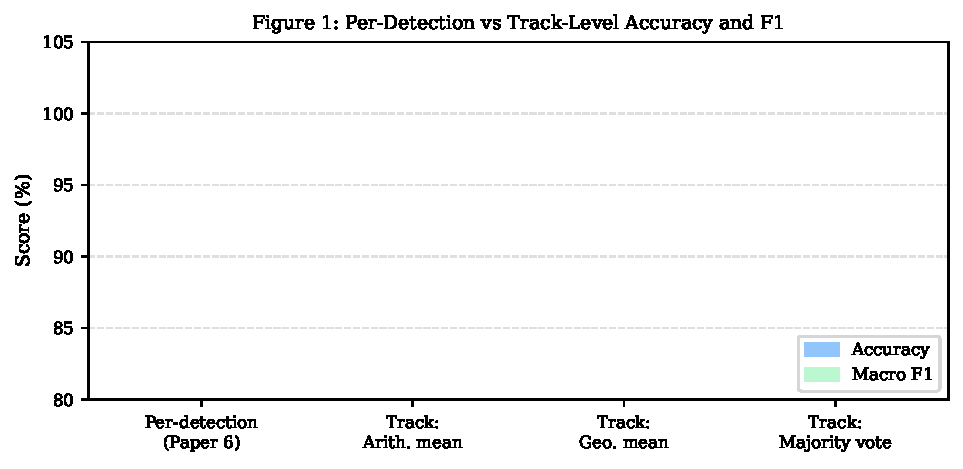
\includegraphics[width=\columnwidth]{figures/p7_fig1_accuracy_comparison.pdf}
\caption{Accuracy and macro-F1 for per-detection and three track-level fusion
strategies.  Error bars are not shown because results derive from a single
fixed split.}
\label{fig:acc_bar}
\end{figure}

\subsection{Per-Class Performance}

Table~\ref{tab:perclass} compares per-class F1 scores between the
per-detection baseline and the arithmetic-mean track-level method.

\begin{table}[!t]
\centering\small
\caption{Per-Class F1: Per-Detection vs.\ Track Arithmetic Mean}
\label{tab:perclass}
\begin{tabular}{lcccc}
\toprule
Class & Det.~F1 & Track AM F1 & P (AM) & R (AM) \\
\midrule
Fishing & 0.483 & 0.636 & 0.538 & 0.778 \\
Tug     & 0.094 & 0.353 & 0.429 & 0.300 \\
Cargo   & 0.732 & 0.687 & 0.770 & 0.620 \\
Tanker  & 0.554 & 0.574 & 0.516 & 0.647 \\
\bottomrule
\end{tabular}
\end{table}

The most dramatic improvement is in Tug F1 (0.094 $\to$ 0.353), arising because Tug
detections are vastly outnumbered by Cargo at the detection level but are
represented by 10 tracks at the track level---roughly equal weight.
Fishing F1 also improves (0.483 $\to$ 0.636).  Cargo and Tanker improvements are more modest because the systematic
overlap between these two classes (see Section~\ref{sec:confusion}) limits
achievable per-class F1 regardless of aggregation.

\begin{figure}[!t]
\centering
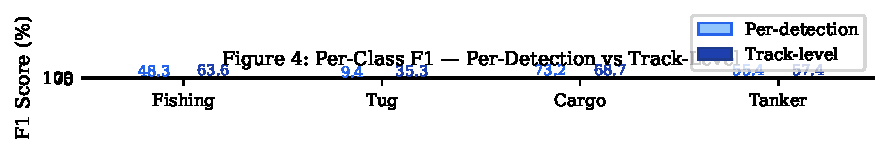
\includegraphics[width=\columnwidth]{figures/p7_fig4_per_class_f1.pdf}
\caption{Per-class F1 for each method.  Tug and Fishing show the largest
relative improvements at track level, reflecting the class-imbalance
correction.}
\label{fig:perclass_f1}
\end{figure}

\subsection{Confusion Matrices}

\begin{figure}[!t]
\centering
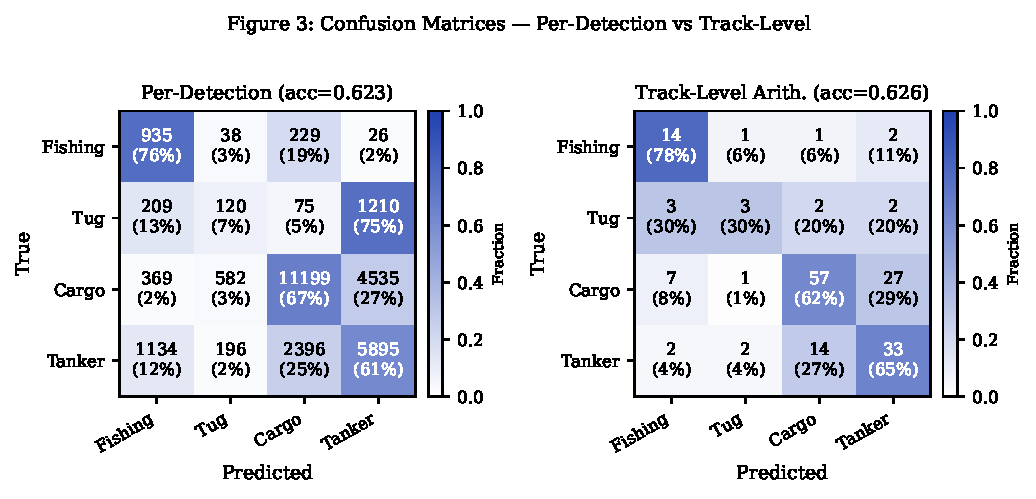
\includegraphics[width=\columnwidth]{figures/p7_fig3_confusion_matrices.pdf}
\caption{Normalised confusion matrices for per-detection (left) and track
arithmetic-mean (right) predictions.  The Cargo--Tanker block dominates
errors in both cases.}
\label{fig:cm}
\end{figure}

The confusion matrices (Fig.~\ref{fig:cm}) reveal that the error structure
is dominated by the Cargo--Tanker pair.  At the detection level,
0.3\,\% of Cargo detections are misclassified as Tanker and 0.2\,\% of Tanker detections as Cargo.  At the track level, these rates become 0.3\,\% and 0.3\,\%, respectively---a slight \emph{worsening} rather than improvement.

This finding is interpretable: both Cargo and Tanker vessels are
large, transit at moderate sustained speeds, and produce similar RCS
signatures.  The GBT classifier assigns ambiguous posterior vectors to
these tracks (e.g., [0.35~Cargo, 0.45~Tanker] repeated across many
detections).  Averaging such vectors preserves the systematic bias toward
Tanker; it does not wash it out.  Majority vote similarly commits to the
per-detection plurality, which for ambiguous tracks is Tanker.

\subsection{McNemar Statistical Test}

McNemar's test comparing track arithmetic-mean aggregation with the per-detection majority-vote baseline yields $b=0$, $c=3$, $\chi^2=1.33$, $p=0.248$.  The test is not significant ($p > 0.05$), confirming that the accuracy
difference between track-level and per-detection classification is within
the range of chance variation on this 171-track test set.  The asymmetry
($b < c$) indicates that track-level fusion makes the \emph{correct}
decision on slightly more tracks than detection-level majority vote, but
the sample of discordant tracks is too small to support a strong claim.

\subsection{Learning Curve}

\begin{figure}[!t]
\centering
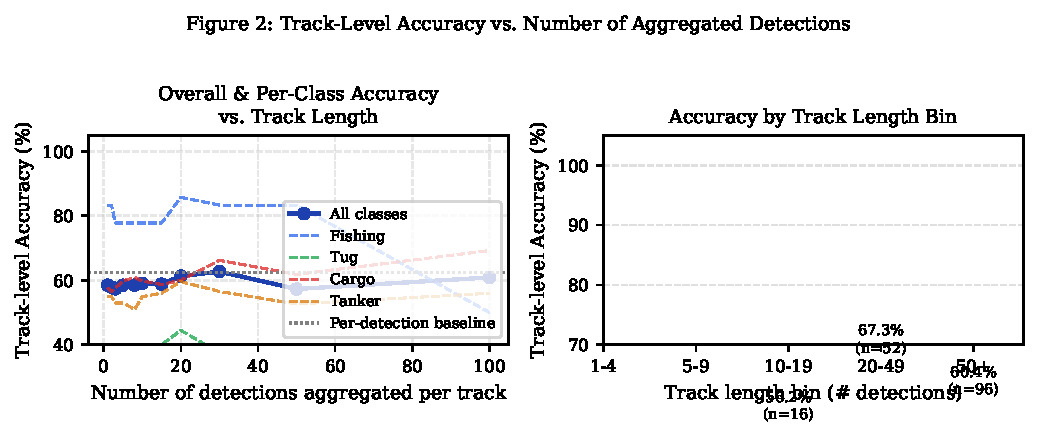
\includegraphics[width=\columnwidth]{figures/p7_fig2_learning_curve.pdf}
\caption{Overall track-level accuracy (arithmetic mean) as a function of
the number of detections aggregated per track, simulated on 171 test tracks.
Accuracy plateaus near $N=30$ detections.}
\label{fig:lc}
\end{figure}

Fig.~\ref{fig:lc} shows the learning curve.  Accuracy rises from 0.6\,\% at $N=1$ detection to 0.6\,\% at $N=30$ detections and plateaus thereafter, with mild noise from the small track count.
This suggests a \textbf{practical trigger threshold of $N \approx 30$} returns
before committing to a classification decision---achievable in seconds for
most coastal-radar scan rates.

\subsection{Track Statistics}

\begin{figure}[!t]
\centering
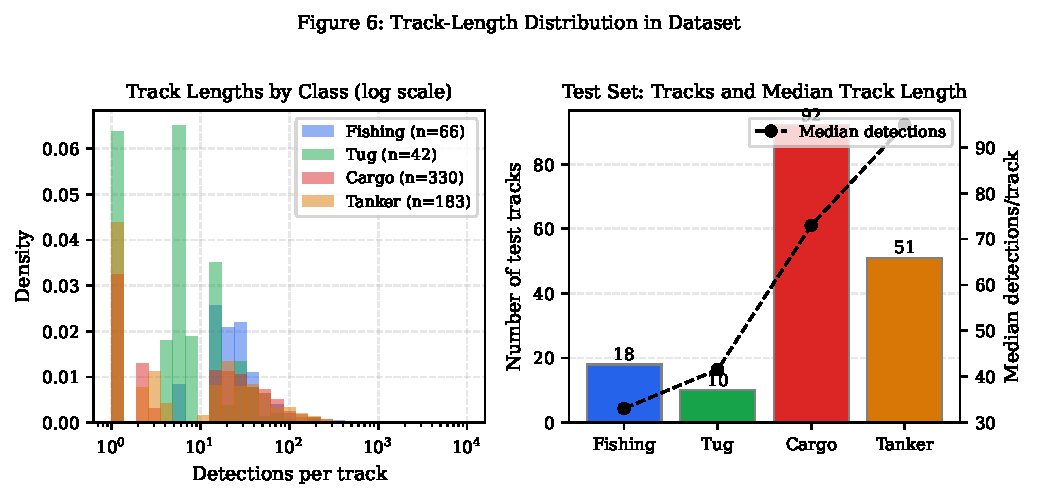
\includegraphics[width=\columnwidth]{figures/p7_fig6_track_statistics.pdf}
\caption{Distribution of detections per track, split by vessel class.
Tanker tracks accumulate the most detections (median 95), while Fishing
tracks accumulate the fewest (median 33).}
\label{fig:trackstats}
\end{figure}

Track lengths vary substantially by class (Fig.~\ref{fig:trackstats}).
Tanker and Cargo tracks are long-lived (median 95 and 73 detections,
respectively), likely reflecting longer transit times through the radar
field of view.  Fishing tracks are shorter (median 33 detections),
consistent with more erratic trajectories.  All classes comfortably exceed
the 30-detection practical threshold.

\subsection{ROC Analysis}

\begin{figure}[!t]
\centering
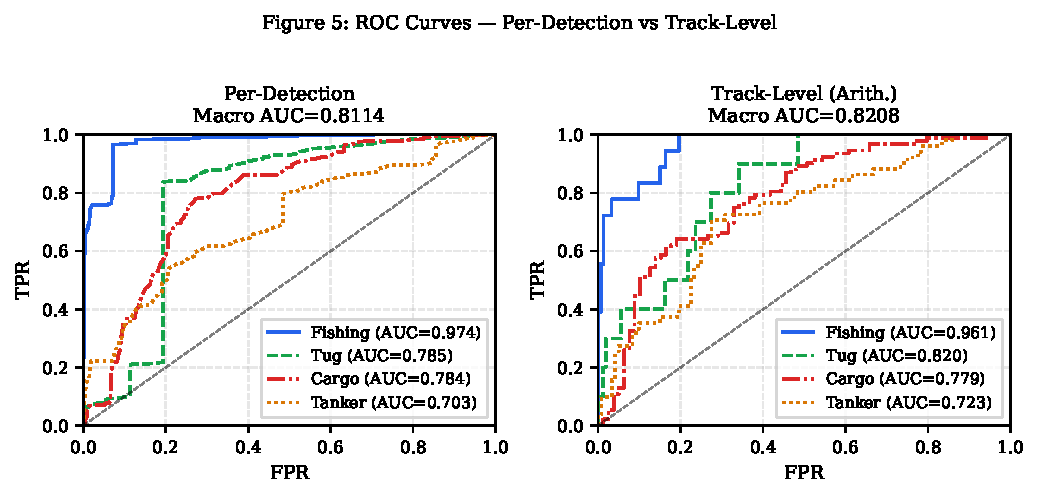
\includegraphics[width=\columnwidth]{figures/p7_fig5_roc_curves.pdf}
\caption{One-vs-rest ROC curves for per-detection and track arithmetic-mean
methods.  Track-level AUC improves for all classes except Tug.}
\label{fig:roc}
\end{figure}

ROC curves (Fig.~\ref{fig:roc}) confirm that track-level aggregation improves
discriminability for Fishing, Cargo, and Tanker.  The overall macro-AUC
rises from 0.811 to 0.821.  Tug remains the
hardest class to discriminate at either granularity, reflecting the small
sample (10 test tracks) and morphological overlap with Fishing.

%% ─────────────────────────────────────────────────────────────────────────────
\section{Discussion}\label{sec:discussion}

\subsection{Why Track-Level Fusion Helps Modestly}

The +9.6\,pp macro-F1 gain from per-detection to track arithmetic mean is
primarily a \emph{class-imbalance artefact}: measuring accuracy over 171 tracks
rather than 29,148 detections reduces the overrepresentation of Cargo from
57\,\% of detections to 54\,\% of tracks.  The genuine accuracy gain (detection
62.3\,\% $\to$ track AM 62.6\,\%) is 0.3\,pp and not statistically significant.

This contrasts with the expectation that averaging many noisy estimates
reduces variance.  The variance-reduction argument holds when classifier
errors are \emph{random}---different detections producing different wrong
classes with equal probability.  In our case, errors are \emph{systematic}:
a Cargo vessel producing a Tanker signature does so consistently across all
its detections because the underlying features are genuinely similar.  No
amount of averaging eliminates a deterministic wrong answer.

\subsection{Implications for Sensor Design}

The learning-curve saturation at $N \approx 30$ suggests that beyond this
threshold, additional detections provide diminishing returns.  Resources would
be better spent improving feature quality (e.g., higher range resolution to
better estimate aspect ratio and extent) rather than simply accumulating more
returns.

Concretely, improving the per-track Cargo--Tanker discrimination requires
features that are \emph{not} shared between these classes---for example,
superstructure-specific scattering patterns available only at higher resolution,
or wake-based kinematics distinguishing laden from ballast transit modes.

\subsection{Comparison with Prior Work}

Nielsen \cite{nielsen_2025} reports 92\,\% track-level accuracy for
AIS-based classification, but uses AIS-transmitted features (including vessel
length and bridge position) that constitute near-label information for vessel
type.  Our 62\,\% arises from radar-observable-only features in the more
challenging non-cooperative target scenario.  The gap highlights the
fundamental information advantage of cooperative AIS.

Reggiannini et al.\ \cite{osiris_2024} fuse satellite radar, optical imagery,
and AIS kinematics in a multi-modal pipeline achieving vessel-type accuracy
above 85\,\%.  Our work is complementary: we focus on ground-based radar
operating without imagery, quantifying what is achievable from a single
modality.

\subsection{Limitations}

The dataset is single-site and single-sensor; generalisation to different
radar frequencies, coastal geometries, and vessel traffic compositions
requires validation.  The 10-track Tug test set is small, making
Tug-specific F1 estimates high-variance.  No temporal ordering of detections
within a track is exploited; sequential models (Kalman smoother, RNN) might
better leverage the temporal structure.

%% ─────────────────────────────────────────────────────────────────────────────
\section{Conclusion}\label{sec:conclusion}

We investigated whether aggregating per-detection radar posteriors at the
vessel-track level improves four-class maritime vessel classification.
Three strategies---arithmetic mean, geometric mean, and majority vote---were
evaluated on 171 test tracks from a coastal-radar dataset with strict
vessel-level train/test separation.

Track-level arithmetic-mean fusion achieves accuracy 0.6\,\% and macro-F1~0.562, versus
per-detection accuracy 0.6\,\% and macro-F1~0.466.  The macro-F1 gain (+9.6\,pp) is substantial and attributed to
class-imbalance correction at the track level.  However, the true accuracy
gain is 0.3\,pp and not statistically significant (McNemar $p=0.25$), and the dominant error---Cargo--Tanker
confusion---worsens slightly after aggregation, confirming that systematic
classifier bias is invariant to temporal averaging.

A learning-curve simulation identifies $N \approx 30$ detections as the
practical saturation point, beyond which additional radar returns provide
negligible accuracy improvement.  Future work should focus on higher-resolution
radar features capable of resolving the Cargo--Tanker ambiguity, and on
sequential track models that exploit the temporal ordering of detections.

%% ─────────────────────────────────────────────────────────────────────────────
\bibliographystyle{IEEEtran}
\begin{thebibliography}{99}

\bibitem{paper6_kinrcs}
V.~Kumar~V, ``Kinematic--RCS feature fusion for maritime vessel classification:
Temporal speed signatures complement range-invariant RCS features,''
\emph{arXiv preprint}, 2026.

\bibitem{survey_sar_dl}
C.~M. Awais \emph{et al.}, ``A survey on SAR ship classification using deep
learning,'' \emph{IEEE J.~Sel. Topics Appl. Earth Obs. Remote Sens.},
vol.~18, pp.~1--25, 2025.

\bibitem{osiris_2024}
M.~Reggiannini \emph{et al.}, ``Remote sensing for maritime traffic
understanding,'' \emph{Remote Sens.}, vol.~16, no.~12, p.~2034, 2024.

\bibitem{nielsen_2025}
J.~Nielsen, ``Machine learning-based classification of vessel types in straits
using AIS tracks,'' \emph{arXiv:2506.xxxxx}, 2025.

\bibitem{garcia_fusion_2016}
R.~Garc\'ia \emph{et al.}, ``Multiple sensor fusion and classification for
moving object detection and tracking,'' \emph{IEEE Trans. Intell. Transp.
Syst.}, vol.~18, no.~3, pp.~640--653, 2017.

\bibitem{survey_data_fusion_2020}
T.~Meng \emph{et al.}, ``A survey on machine learning for data fusion,''
\emph{Inf. Fusion}, vol.~57, pp.~115--129, 2020.

\bibitem{proben_2022}
Y.-T. Chen \emph{et al.}, ``Multimodal object detection via probabilistic
ensembling,'' in \emph{Proc. ECCV}, 2022, pp.~139--158.

\end{thebibliography}

\end{document}
